\documentclass[../main.tex]{subfiles}
\graphicspath{{\subfix{../images/}}}
\begin{document}

\hypertarget{exacttriganswers}{\subsection*{Answers - Exact trig values (\hyperlink{exacttriglink}{page \pageref{Exact trig values}})}}

\label{Exact trig values answers}
\begin{enumerate}[itemsep=0.4cm]
    \item 
    $\cos{45}=\frac{1}{\sqrt{2}}=\frac{\sqrt{2}}{2}$

    \item 
    $\sin{105}=\sin{(60+45)}=\sin{60}\cos{45}+\cos{60}\sin{45}$

    $=\frac{\sqrt{3}}{2}\times \frac{1}{\sqrt{2}}+\frac{1}{2}\times \frac{1}{\sqrt{2}}$

    $=\frac{\sqrt{3}+1}{2\sqrt{2}}$

    Rationalising by multiplying by $\frac{\sqrt{2}}{\sqrt{2}}$:

    $=\frac{\sqrt{6}+\sqrt{2}}{4}$

    \item 
    $\tan{60}=\sqrt{3}$

    \item 
    $\cos{\frac{7\pi}{12}}=\cos{\Bigl(\frac{4\pi}{12}+\frac{3\pi}{12}\Bigr)}=\cos{\Bigl(\frac{\pi}{3}+\frac{\pi}{4}\Bigr)}$

    $=\cos{\Bigl(\frac{\pi}{3}}\Bigr)\cos{\Bigl(\frac{\pi}{4}}\Bigr)-\sin{\Bigl(\frac{\pi}{3}}\Bigr)\sin{\Bigl(\frac{\pi}{4}}\Bigr)$

    $=\frac{1}{2}\times \frac{1}{\sqrt{2}}-\frac{\sqrt{3}}{2}\times \frac{1}{\sqrt{2}}$

    $=\frac{1-\sqrt{3}}{2\sqrt{2}}$

    Rationalise by multiplying by $\frac{\sqrt{2}}{\sqrt{2}}$

    $=\frac{\sqrt{2}-\sqrt{6}}{4}$

    \item 
    $\cos{\frac{\pi}{12}}=\cos{\Bigl(\frac{4\pi}{12}-\frac{3\pi}{12}\Bigr)}=\cos{\Bigl(\frac{\pi}{3}-\frac{\pi}{4}\Bigr)}$

    $=\cos{\Bigl(\frac{\pi}{3}}\Bigr)\cos{\Bigl(\frac{\pi}{4}}\Bigr)+\sin{\Bigl(\frac{\pi}{3}}\Bigr)\sin{\Bigl(\frac{\pi}{4}}\Bigr)$

    $=\frac{1}{2}\times \frac{1}{\sqrt{2}}+\frac{\sqrt{3}}{2}\times \frac{1}{\sqrt{2}}$

    $=\frac{1+\sqrt{3}}{2\sqrt{2}}$

    Rationalise by multiplying by $\frac{\sqrt{2}}{\sqrt{2}}$

    $=\frac{\sqrt{2}+\sqrt{6}}{4}$

    \item 
    $\tan{\Bigl(\frac{2\pi}{3}\Bigr)}=\tan{\Bigl(2\times \frac{\pi}{3}\Bigr)}$

    $=\frac{2\tan\Bigl(\frac{\pi}{3}\Bigr)}{1-\tan^2{\Bigl(\frac{\pi}{3}\Bigr)}}$

    $=\frac{2\times \sqrt{3}}{1-(\sqrt{3})^2}$

    $=\frac{2\sqrt{3}}{1-3}=\frac{2\sqrt{3}}{-2}=-\sqrt{3}$

    \item 
    $\cos\Bigl(\frac{5\pi}{12}\Bigr)=\cos{\Bigl(\frac{\pi}{6}+\frac{\pi}{4}\Bigr)}$

    $=\cos{(\frac{\pi}{6})}\cos{(\frac{\pi}{4})}-\sin{(\frac{\pi}{6})}\sin{(\frac{\pi}{4})}$

    $=\frac{\sqrt{3}}{2}\times \frac{1}{\sqrt{2}}-\frac{1}{2}\times \frac{1}{\sqrt{2}}$

    $=\frac{\sqrt{3}-1}{2\sqrt{2}}$

    Rationalising by multiplying by $\frac{\sqrt{2}}{\sqrt{2}}$:

    $=\frac{\sqrt{6}-\sqrt{2}}{4}$

    \item 
    $\sin{\Bigl(-\frac{4\pi}{3}\Bigr)}=-\sin{\Bigl(\frac{4\pi}{3}\Bigr)}$
    (Since sine is an odd function)

    $=-\sin{\Bigl(\pi + \frac{\pi}{3}\Bigr)}$

    $=-\Bigl(\sin{(\pi)}\cos{(\frac{\pi}{3})}+\cos{(\pi)}\sin{(\frac{\pi}{3})}\Bigr)$

    $=-\Bigl(0-\frac{\sqrt{3}}{2}\Bigr)$

    $=\frac{\sqrt{3}}{2}$

    \item 
    $\sin{\Bigl(\frac{7\pi}{12}\Bigr)}=\sin{\Bigl(2\pi-\frac{\pi}{4}\Bigr)}$

    $=\sin{(2\pi)}\cos{\Bigl(\frac{\pi}{4}\Bigr)}-\cos{(2\pi)}\sin{\Bigl(\frac{\pi}{4}\Bigr)}$

    $=0-\frac{1}{\sqrt{2}}$

    $=-\frac{1}{\sqrt{2}}$

    $=-\frac{\sqrt{2}}{2}$

    \item 
    $\tan{\Bigl(\frac{3\pi}{4}\Bigr)}=\tan{\Bigl(\pi-\frac{\pi}{4}\Bigr)}$

    $=\frac{\tan{(\pi)}-\tan{(\frac{\pi}{4})}}{1-\tan{(\pi)}\tan{(\frac{\pi}{4})}}$

    $=\frac{0-1}{1-0\times 1}$

    $=-1$

    \item 
    $\theta = 18$

    $5\theta = 90$

    $2\theta +3\theta = 90$

    $2\theta = 90 - 3\theta$

    $\sin{2\theta}=\sin{(90 - 3\theta)}$

    $2\sin{\theta}\cos{\theta}=\sin{90}\cos{3\theta}-\cos{90}\sin{3\theta}$

    $2\sin{\theta}\cos{\theta}=\cos{3\theta}$

    $2\sin{\theta}\cos{\theta}=\cos{(2\theta + \theta)}$

    $2\sin{\theta}\cos{\theta}=\cos{2\theta}\cos{\theta}-\sin{2\theta}\sin{\theta}$

    Use double angle rules for both cosine and sine:

    $2\sin{\theta}\cos{\theta}=(1-2\sin^2{\theta})\cos{\theta}-2\sin^2{\theta}\cos{\theta}$

    Divide through by $\cos{\theta}$:

    $2\sin{\theta}=(1-2\sin^2{\theta})-2\sin^2{\theta}$

    $2\sin{\theta}=1-4\sin^2{\theta}$

    Form a quadratic and solve:

    $4\sin^2{\theta}+2\sin{\theta}-1=0$

    $\sin{\theta}=\frac{-2\pm \sqrt{20}}{8}=\frac{-2\pm 2\sqrt{5}}{8}=\frac{-1\pm \sqrt{5}}{4}$

    Because we know $\sin{18}$ is positive we can disregard the negative solution:

    $\sin{18}=\frac{-1+\sqrt{5}}{4}$

    Using a right-angle triangle we can now find the value of $\cos{18}$

    \begin{figure}[h]
        \centering
        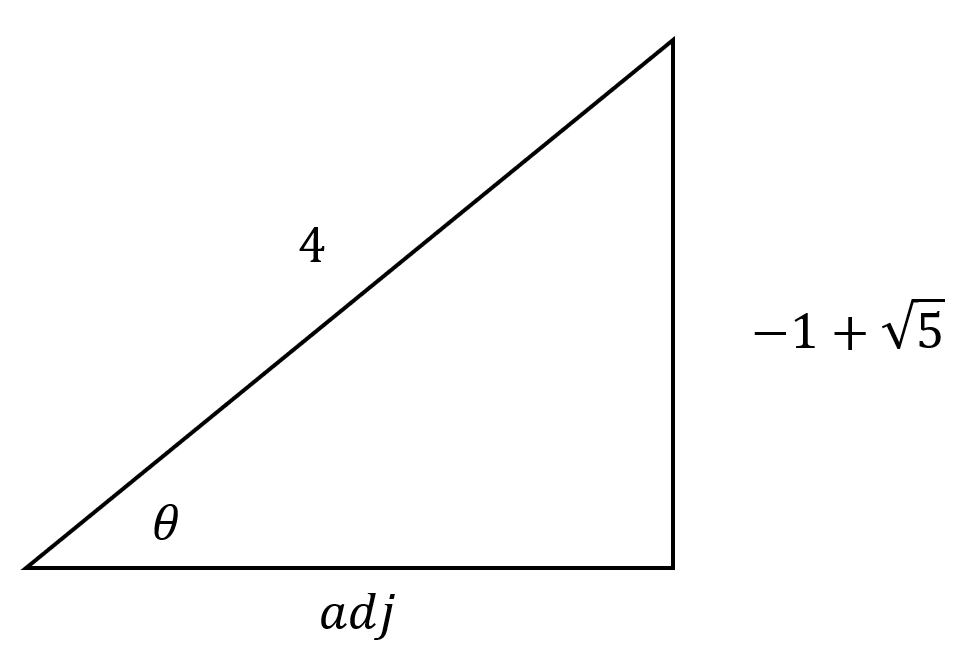
\includegraphics[width=0.5\textwidth]{images/exacttrigvalues11.png}
    \end{figure}

    $(adj)^2=4^2-(-1+\sqrt{5})^2$

    $(adj)^2=10+2\sqrt{5}$

    $adj=\sqrt{10+2\sqrt{5}}$

    $\cos{18}=\frac{\sqrt{10+2\sqrt{5}}}{4}$

    \item 
    $\theta = 36$

    $5\theta = 180$

    $2\theta + 3\theta = 180$

    $2\theta = 180 - 3\theta$

    $\sin{2\theta} = \sin{(180-3\theta)}$

    $2\sin{\theta}\cos{\theta}=\sin{180}\cos{3\theta}-\cos{180}\sin{3\theta}$

    $2\sin{\theta}\cos{\theta}=\sin{3\theta}$

    $2\sin{\theta}\cos{\theta}=\sin{(2\theta+\theta)}$

    $2\sin{\theta}\cos{\theta}=\sin{2\theta}\cos{\theta}+\cos{2\theta}\sin{\theta}$

    Use double angles rules for both sine and cosine:

    $2\sin{\theta}\cos{\theta}=2\sin{\theta}\cos^2{\theta}+(2\cos^2{\theta}-1)\sin{\theta}$

    Divide through by $\sin{\theta}$:

    $2\cos{\theta}=2\cos^2{\theta}+(2\cos^2{\theta}-1)$

    Form a quadratic:

    $4\cos^2{\theta}-2\cos{\theta}-1=0$

    $\cos{\theta}=\frac{2\pm \sqrt{20}}{8}$

    Since we know that $\cos{36}$ is positive, we can ignore the negative:

    $\cos{\theta}=\cos{36}=\frac{1+\sqrt{5}}{4}$

    We can use this to find $\sin{36}$ by substituting into a right-angle triangle:

    \begin{figure}[h]
        \centering
        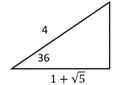
\includegraphics[width=0.15\linewidth]{images/exacttrigvalues.png}
    \end{figure}

    Now we can use Pythagoras to find the opposite side, which then can be used to find $\sin{36}$:

    Opposite = $\sqrt{4^2-(1+\sqrt{5})^2}=\sqrt{10-2\sqrt{5}}$

    This means that $\sin{36}=\frac{O}{H}=\frac{\sqrt{10-2\sqrt{5}}}{4}$

    \item 
    $\theta=\frac{2\pi}{5}$

    $5\theta=2\pi$

    $2\theta=2\pi - 3\theta$

    $\sin{2\theta}=\sin{(2\pi-3\theta)}$

    $2\sin{\theta}\cos{\theta}=\sin{2\pi}\cos{3\theta}-\cos{2\pi}\sin{3\theta}$

    $2\sin{\theta}\cos{\theta}=-\sin{3\theta}$

    $2\sin{\theta}\cos{\theta}=-\sin{(2\theta+\theta)}$

    $2\sin{\theta}\cos{\theta}=-(\sin{2\theta}\cos{\theta}+\cos{2\theta}\sin{\theta})$

    $2\sin{\theta}\cos{\theta}=-2\sin{\theta}\cos^2{\theta}-(2\cos^2{\theta}-1)\sin{\theta}$

    Divide through by $\sin{\theta}$:

    $2\cos{\theta}=-2\cos^2{\theta}-(2\cos^2{\theta}-1)$

    Form a quadratic:

    $4\cos^{\theta}+2\cos{\theta}-1=0$

    $\cos{\theta}=\cos{\Bigl(\frac{2\pi}{5}\Bigr)}=\frac{-2\pm \sqrt{20}}{8}=\frac{-1\pm \sqrt{5}}{4}$

    We can use this to find $\sin{\frac{2\pi}{5}}$ by substituting it into a right-angle triangle:

    \begin{figure}[h]
        \centering
        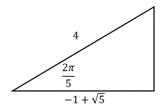
\includegraphics[width=0.2\linewidth]{images/exacttrigvalues2.png}
    \end{figure}

    Now we can use Pythagoras to find the opposite side, which then can be used to find $\sin{\frac{2\pi}{5}}$

    Opposite = $\sqrt{4^2-(-1+\sqrt{5})^2}=\sqrt{10+2\sqrt{5}}$

    This means $\sin{\frac{2\pi}{5}}=\frac{O}{H}=\frac{\sqrt{10+2\sqrt{5}}}{4}$
\end{enumerate}




\end{document}